\section{Inherently Non-resonant Antenna}
In this section the prototype of the Inherently non-resonant antenna will be described.

The prototype is shown in Figure. 

   \begin{table}
      \centering
      \begin{tabular}{|l|l|r|r|r|}
        \hline
        Antenna & Band & Start [MHz] & Stop [MHz] & Bandwidth [MHz] \\
        \hline
        Top     & Low  & 690        & 870       & 180 \\
        Side    & Low  & 710         & 1050        & 340 \\
        \hline
        Top     & High & 2250        & 2750       & 500 \\
        Side    & High & 2280        & 3000       & 720 \\
        \hline
      \end{tabular}
      \caption{Maximum bandwidth obtained in the low and high band for the top and the side antenna, respectively.}
      \label{tab:bw_sol3_proto}
    \end{table}

\subsection{Measurement and Simulation Comparison}
\fixme{plot sim and meas comparison}


\section{Capacitor sweep}
\begin{figure}[htbp]
    \centering
    \begin{subfigure}{0.49\linewidth}
        \centering
        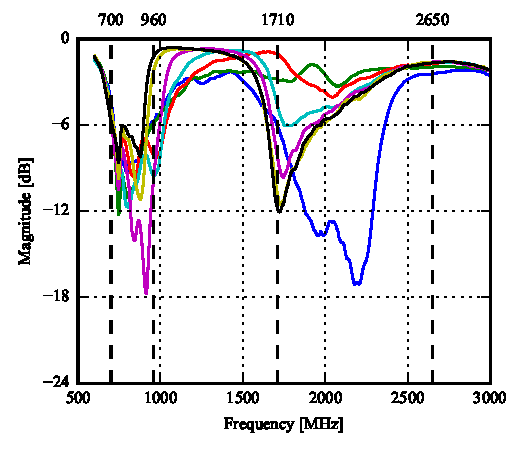
\includegraphics{img/tech_sol/nonresonant/prototype/s11_csh1.pdf}
        \caption{$S_{11}$, sweeping the top antenna and fixing the side antenna.}
    \end{subfigure}
    \hfill
    \begin{subfigure}{0.49\linewidth}
        \centering
        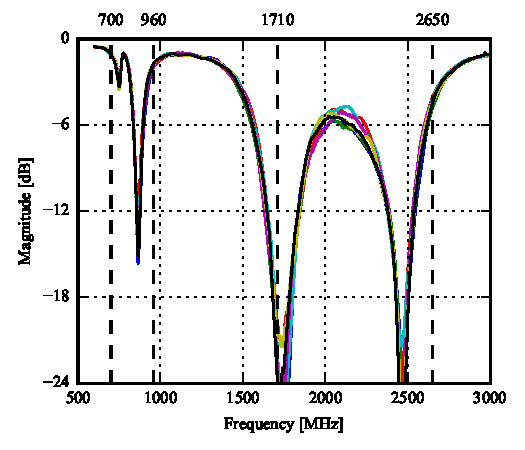
\includegraphics{img/tech_sol/nonresonant/prototype/s22_csh1.pdf}
        \caption{$S_{22}$, sweeping the side antenna and fixing the top antenna.}
    \end{subfigure}
    \\
    \begin{subfigure}{0.49\linewidth}
        \centering
        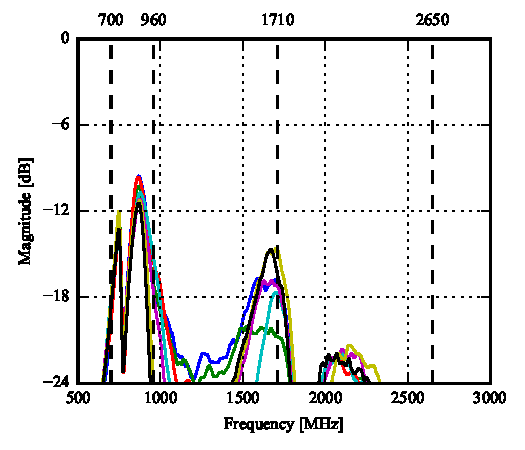
\includegraphics{img/tech_sol/nonresonant/prototype/s21_csh1.pdf}
        \caption{$S_{21}$, sweeping the top antenna and fixing the side antenna.}
    \end{subfigure}
    \hfill
    \begin{subfigure}{0.49\linewidth}
        \centering
        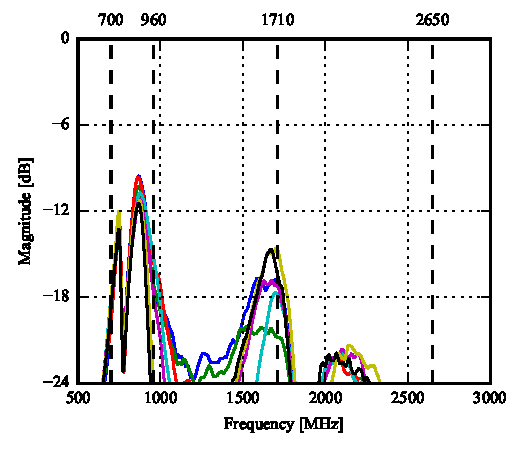
\includegraphics{img/tech_sol/nonresonant/prototype/s12_csh1.pdf}
        \caption{$S_{21}$, sweeping the side antenna and fixing the top antenna.}
    \end{subfigure}
    \caption{Non-resonant antenna. S-parameters for different shunt-capacitor values.}
    \label{fig:nonresonant_proto_sweep_sparams}
\end{figure}